\PassOptionsToPackage{dvipsnames}{xcolor}
\documentclass[a4paper,11pt]{report} %article

\usepackage{graphicx,subfigure,afterpage,hyperref,xspace,xcolor,caption,soul,geometry,pdfpages,stackengine,eso-pic,fancyhdr,hyphenat}


%\usepackage[utf8]{inputenc} %to make the single quote appear correct after the encoding inserted above!

%command to substitute "{\em MyTaxyService}" with "\mts"
\newcommand{\mts}{\mbox{\normalfont\itshape myTaxiService}}
\geometry{margin=1in}

%header & footer style
\fancyhead{}
\fancyhead[C]{\iffloatpage{}{\slshape\rightmark}}
\fancyfoot{}
\fancyfoot[C]{\iffloatpage{}{\thepage}}
\renewcommand{\headrulewidth}{\iffloatpage{0pt}{0.4pt}}
\renewcommand{\footrulewidth}{\iffloatpage{0pt}{0.4pt}}
\pagestyle{fancy}
\renewcommand{\sectionmark}[1]{\markright{\thesection.\ #1}}
\renewcommand{\subsectionmark}[1]{\markright{\thesubsection.\ #1}}

%tOC style: sections bold 
\usepackage[subfigure]{tocloft}
\renewcommand{\cftsecfont}{\bfseries}
\renewcommand{\cftsecpagefont}{\normalfont\bfseries}% page numbers in bold
\renewcommand{\cftdotsep}{1}
\renewcommand{\cftsecleader}{\bfseries\cftdotfill{\cftsecdotsep}}% dot leaders in bold

%to keep the links of the TOC invisible
\hypersetup{
	colorlinks,
	citecolor=black,
	filecolor=black,
	linkcolor=black,
	urlcolor=black
}


\title{Politecnico di Milano\\A.A. 2015/2016\\Software Engineering 2: ``{\em myTaxyService}'' \\ \bigskip 
\textbf{D}esign \textbf{D}ocument}
\author{Alessandro Baldassari (mat. 841561) \\ Alberto Bendin (mat. 841734) \\ Francesco Giarola (mat. 840554)}


%to set the nested bullet lists style
%\renewcommand{\labelitemii}{$\circ$}
\renewcommand{\labelitemii}{}
\renewcommand{\labelitemiii}{$\diamond$}

%to avoid the hyphenation of the name of the software
\hyphenation{myTaxyService}

\begin{document}
	
	%fIRSTPAGE
	
	%pOLIMI-LOGO
	\begin{figure}[t]
		\centering
		\includegraphics[width=1\linewidth]{"Pictures/polimi-logo"}
		\label{fig:polimi-logo}
	\end{figure}
	
	\maketitle
		
	
	%bLANK-PAGE
	\thispagestyle{empty}
	\clearpage\mbox{}\clearpage

	
	
	
	%to number the section from 1 instead of 0.1 with the report class, without using the article class. Avoid the forced use of chapters to number from 1. Tailored for REPORT class!!!
	\renewcommand*\thesection{\arabic{section}}
	\renewcommand*\thesubsection{\arabic{section}.\arabic{subsection}}
	\renewcommand*\thesubsubsection{%
	\arabic{section}.\arabic{subsection}.\arabic{subsubsection}%
	}
	\setcounter{secnumdepth}{4}
	\setcounter{tocdepth}{4}
		
	
	%to change the page numbering from roman in the toc to arabic
	\pagenumbering{roman}
	\tableofcontents
	\newpage
	\pagenumbering{arabic}
	
	
	%to insert the writing "Page" above page numbers in the TOC
	\addtocontents{toc}{~\hfill\textrm{Page}\par}
	
	\section{Introduction}
	
	\subsection{Purpose} This document presents the architecture on which \mts{} will be developed; it describes the decisions taken during the design process and justifies them. The whole design process is described including also the improvements and modifications to provide additional valuable informations in case of future changes of the architecture structure.
	
	\subsection{Scope} Accordingly to the definition of the architecture design this document will focus on the non functional requirements of \mts{}. 
	Since the system architecture  defines constraints on the implementation this document will  be  used to provide fundamental guidelines in the development phase of \mts{}.\\ \newline
	The system architecture will be organized in three categories corresponding to the functionalities of the different users: passengers, drivers and administrator.
	\begin{itemize}
		\item \textbf{Passengers} \\
		The system allows the user to sign up, login, request or reserve a taxi with the customization of the ride. 
		\item \textbf{Taxi drivers} \\
		The system allows the user to login, set the ``availability'' and accept or reject jobs.
		\item \textbf{Administrator} \\
		The system allows the user to login, manage the drivers' list and supervise the system itself.
	\end{itemize}
	
	\subsection{Definitions, Acronyms, Abbreviations}
	The following acronyms are used in this document:
	\begin{itemize}
		\item JEE: Java Enterprise Edition
		\item RASD: Requirements Analysis and Specification Document
		\item ER: Entity Relationship
		\item EIS: Enterprise Information System
	\end{itemize}
	The following definitions are used in this document:
	
	\subsection{Reference Documents}
	\begin{itemize}
		\item Specification document: myTaxiService project
		\item Template for the Design Document
		\item IEEE Std 1016™-2009 - IEEE Standard on Design Descriptions
		\item Requirements Analysis and Specification Document for \mts{}
	\end{itemize}
	
	\subsection{Document Structure} This  document  specifies  the  architecture  of  the  system  using  different levels of detail. It also describes the architectural decisions and justifies them. The design was  developed  in  a  top-­‐down  way, then the  document  reflects this approach.
	The document is organized in the following sections:
	\begin{enumerate}
		\item Introduction\\
		Provides a synopsis of the architectural descriptions.
		\item Architectural design
		\item Algorithm design
		\item User interface design
		\item Requirements traceability
		\item References
		
	\end{enumerate} 
	
	\section{Architectural Design}
	
	\subsection{Overview} This  section  of  the  design  document  provides  a  general  description  of  the  design  of  the  system  and  its  processes;  it includes  the  general  design  context,  the  general  approach  and  describes  the overall design.\\JEE has a four-tiered architecture divided as shown in the picture below:\\
		\begin{minipage}{\linewidth}
%			\vspace*{-0.35cm}
			\makebox[\linewidth]{
				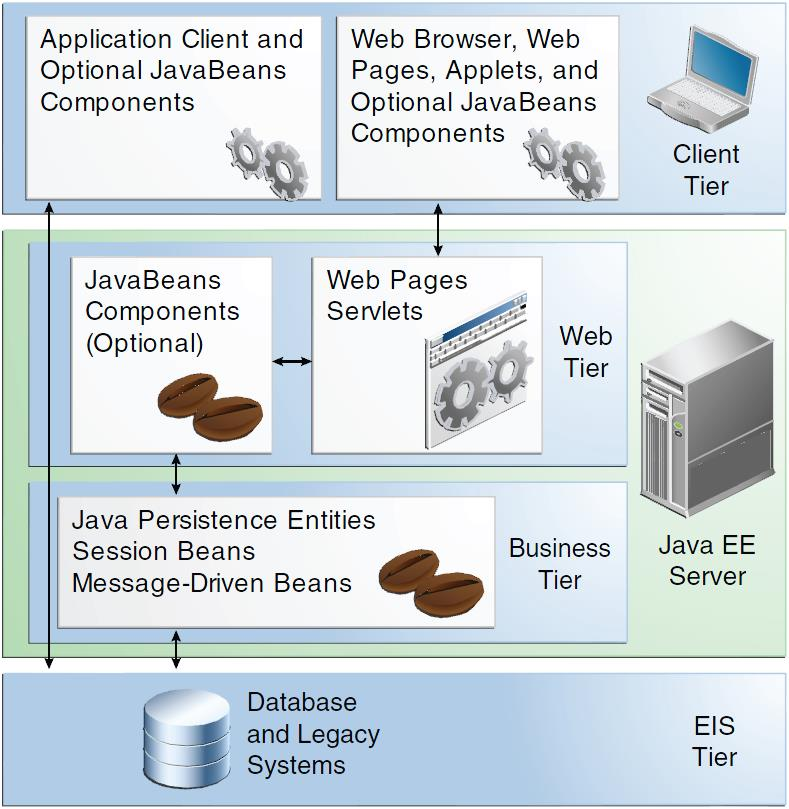
\includegraphics[keepaspectratio=true,scale=0.57]{Pictures/4tier}}
		\end{minipage}	
		\begin{enumerate}
			\item \textbf{Client Tier}: contains Application Clients and Web Browsers and it is the layer designed to interact directly with the actors. This project is a web and mobile application, then the client will use a web browser or a smartphone to access pages.
			\item \textbf{Web Tier}: contains the Servlets and Dynamic Web Pages that needs to be elaborated. This tier receives the requests from the client tier and forwards the pieces of data collected to the business tier waiting for processed data to be sent to the client tier, eventually formatted.
			\item \textbf{Business Tier}: contains the Java Beans, which contain the business logic of the application, and Java Persistence Entities.
			\item \textbf{EIS Tier}: contains the data source. In our case, it is the database allowed to store all the relevant data and to retrieve them.									
		\end{enumerate}
	We can also consider the second and third tier together, in this case the architecture becomes a three-tier one with \textit{client tier}, \textit{business logic tier} and \textit{persistence tier}.\\
	To design the system a top-­‐down approach is used. After the identification of the main three layers, the system is decomposed in components that capture subsets of related functionalities. For each component is specified the role in the architecture and its interactions with the rest of the system. 
	
	\subsection{High level components and their interaction} 
	
	\subsubsection{Identifying sub-systems} We separate the functionalities of our system into these functional areas:
%	\begin{itemize}
%		\item Sign-up
%		\item Login
%		\item User sub-system
%			\begin{itemize}
%				\item Passengers
%				\begin{itemize}
%					\item New request manager
%					\item New reservation manager
%					\item Rides manager
%					\begin{itemize}
%						\item Active rides
%						\item History
%					\end{itemize}
%					\item Profile manager
%					\item Notification manager
%				\end{itemize}
%				\item Taxi drivers
%				\begin{itemize}
%					\item Availability manager
%					\item Jobs manager
%					\item Notification manager
%				\end{itemize}
%				\item Administrator
%				\begin{itemize}
%					\item Drivers manager
%					\begin{itemize}
%						\item Add driver
%						\item Edit driver
%						\item Delete driver
%					\end{itemize}
%				\end{itemize}
%			\end{itemize}
%	\end{itemize}
	\begin{itemize}
		\item myTaxiService
			\begin{itemize}
				\item This component describes the system we were asked to implement.
			\end{itemize} 
		\item Users
			\begin{itemize}
				\item This component represents in general the users that will use the service.
			\end{itemize}
		\item Notification service
			\begin{itemize}
				\item This component represents the notification mechanism our system will use (text-messages, emails and push notifications).
			\end{itemize}
		\item Payment service
			\begin{itemize}
				\item This component represents the external service in charge of managing the payments.
			\end{itemize}
		\item Third party apps
			\begin{itemize}
				\item This component represents in general the external apps that can possibly connect to the system via our public web APIs.
			\end{itemize}
	\end{itemize}
	\hspace{2cm} The following schema shows the above-mentioned components and their interaction.\\
		\begin{minipage}{\linewidth}
			\vspace*{0.35cm}
			\makebox[\linewidth]{
			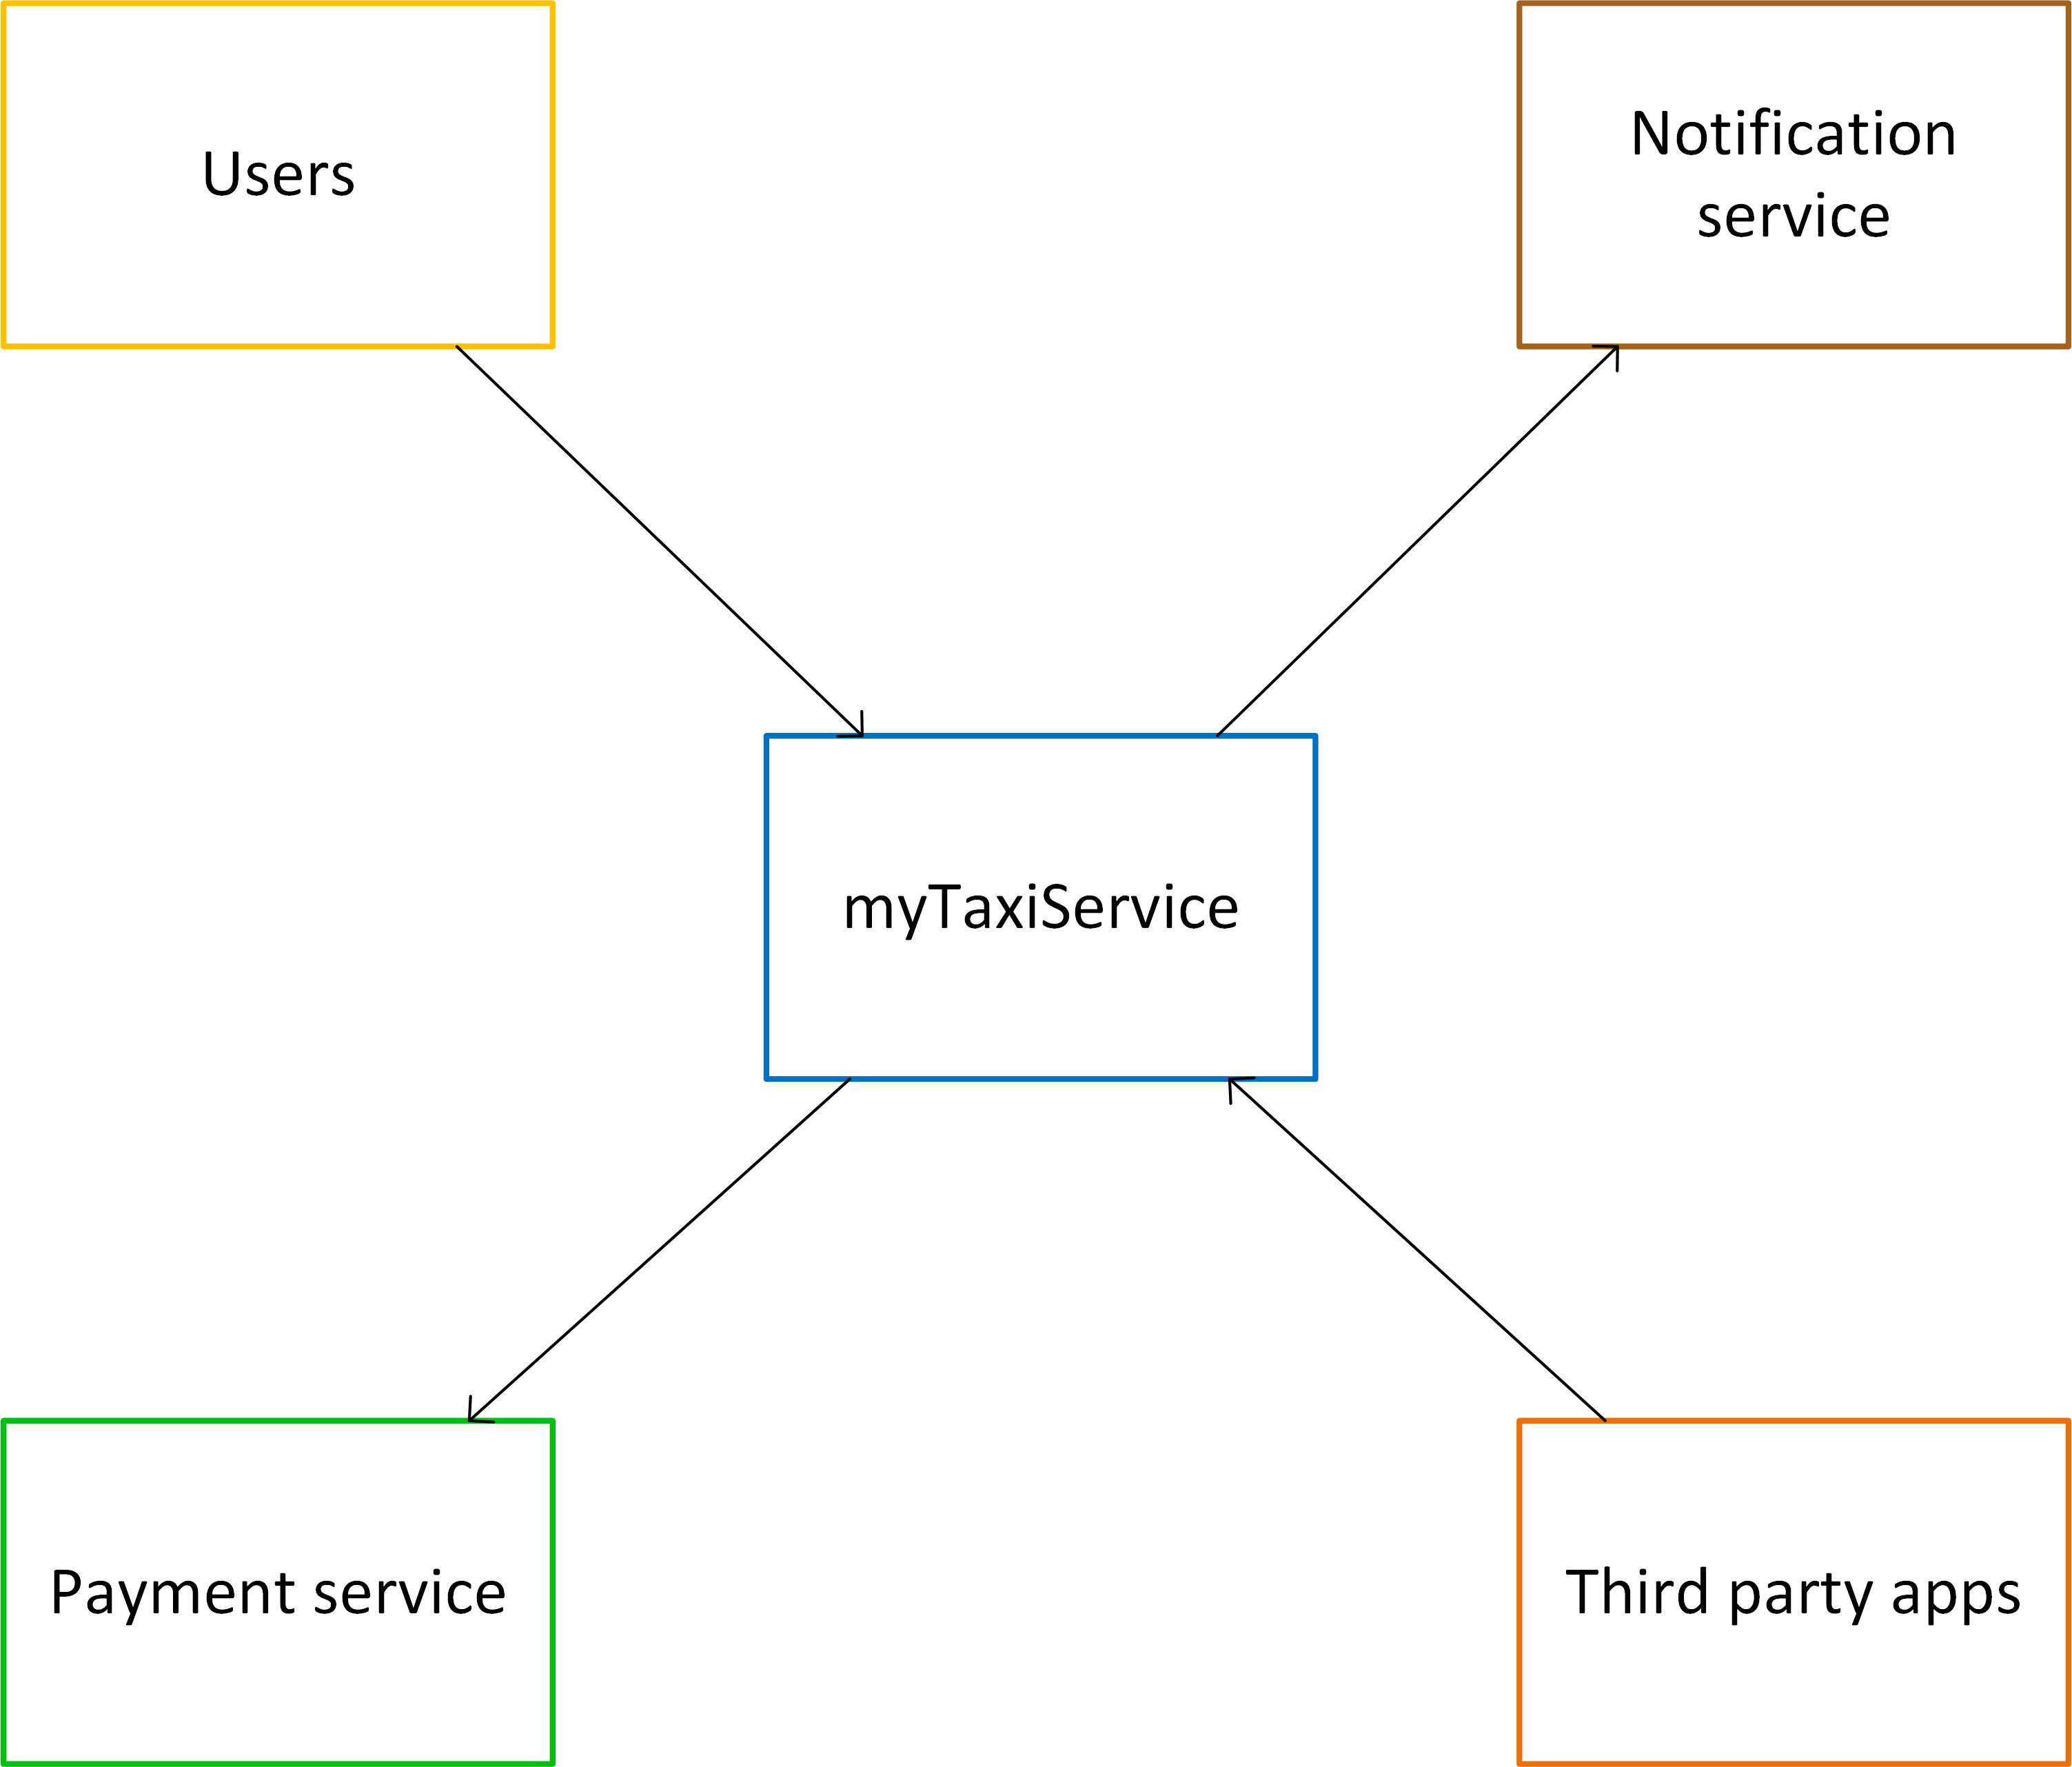
\includegraphics[keepaspectratio=true,scale=0.83]{Pictures/VisioSystemComponentsHighLevel}}
		\end{minipage}
	
%	\subsubsection{General Package design}
%	In this section the general design schemas are presented specifying the basic relations between packages, use cases and users. \\
%	Each layer contains a set of functionalities satisfying the correspondent requirements. Thus we find a mapping between the use cases and the package design of the system.  
%	Considering the three-tier view of the architecture three packages are identified: 
%	\begin{itemize}
%		\item User UI: this  package  is  in  charge  of  interacting  with  the  user; it  obtains  the  user  requests, sends these to the business logic package, obtains the information needed from the latter and displays them to the user accordingly. In general the package contains the user interfaces.
%		\item Business  logic: this package is in charge of receiving and processing the User UI package requests, accessing the Persistence package when needed and sending a response accordingly. 
%		\item Persistence: this package is in charge of managing the data request from the Business logic package.
%	\end{itemize}
%	The  main  users:  Administrator,  passengers  and  taxi  drivers  directly  access the  User  UI  package  but  cannot see the other packages. \\
%	\begin{minipage}{\linewidth}
%%		\vspace*{-0.35cm}
%		\makebox[\linewidth]{
%		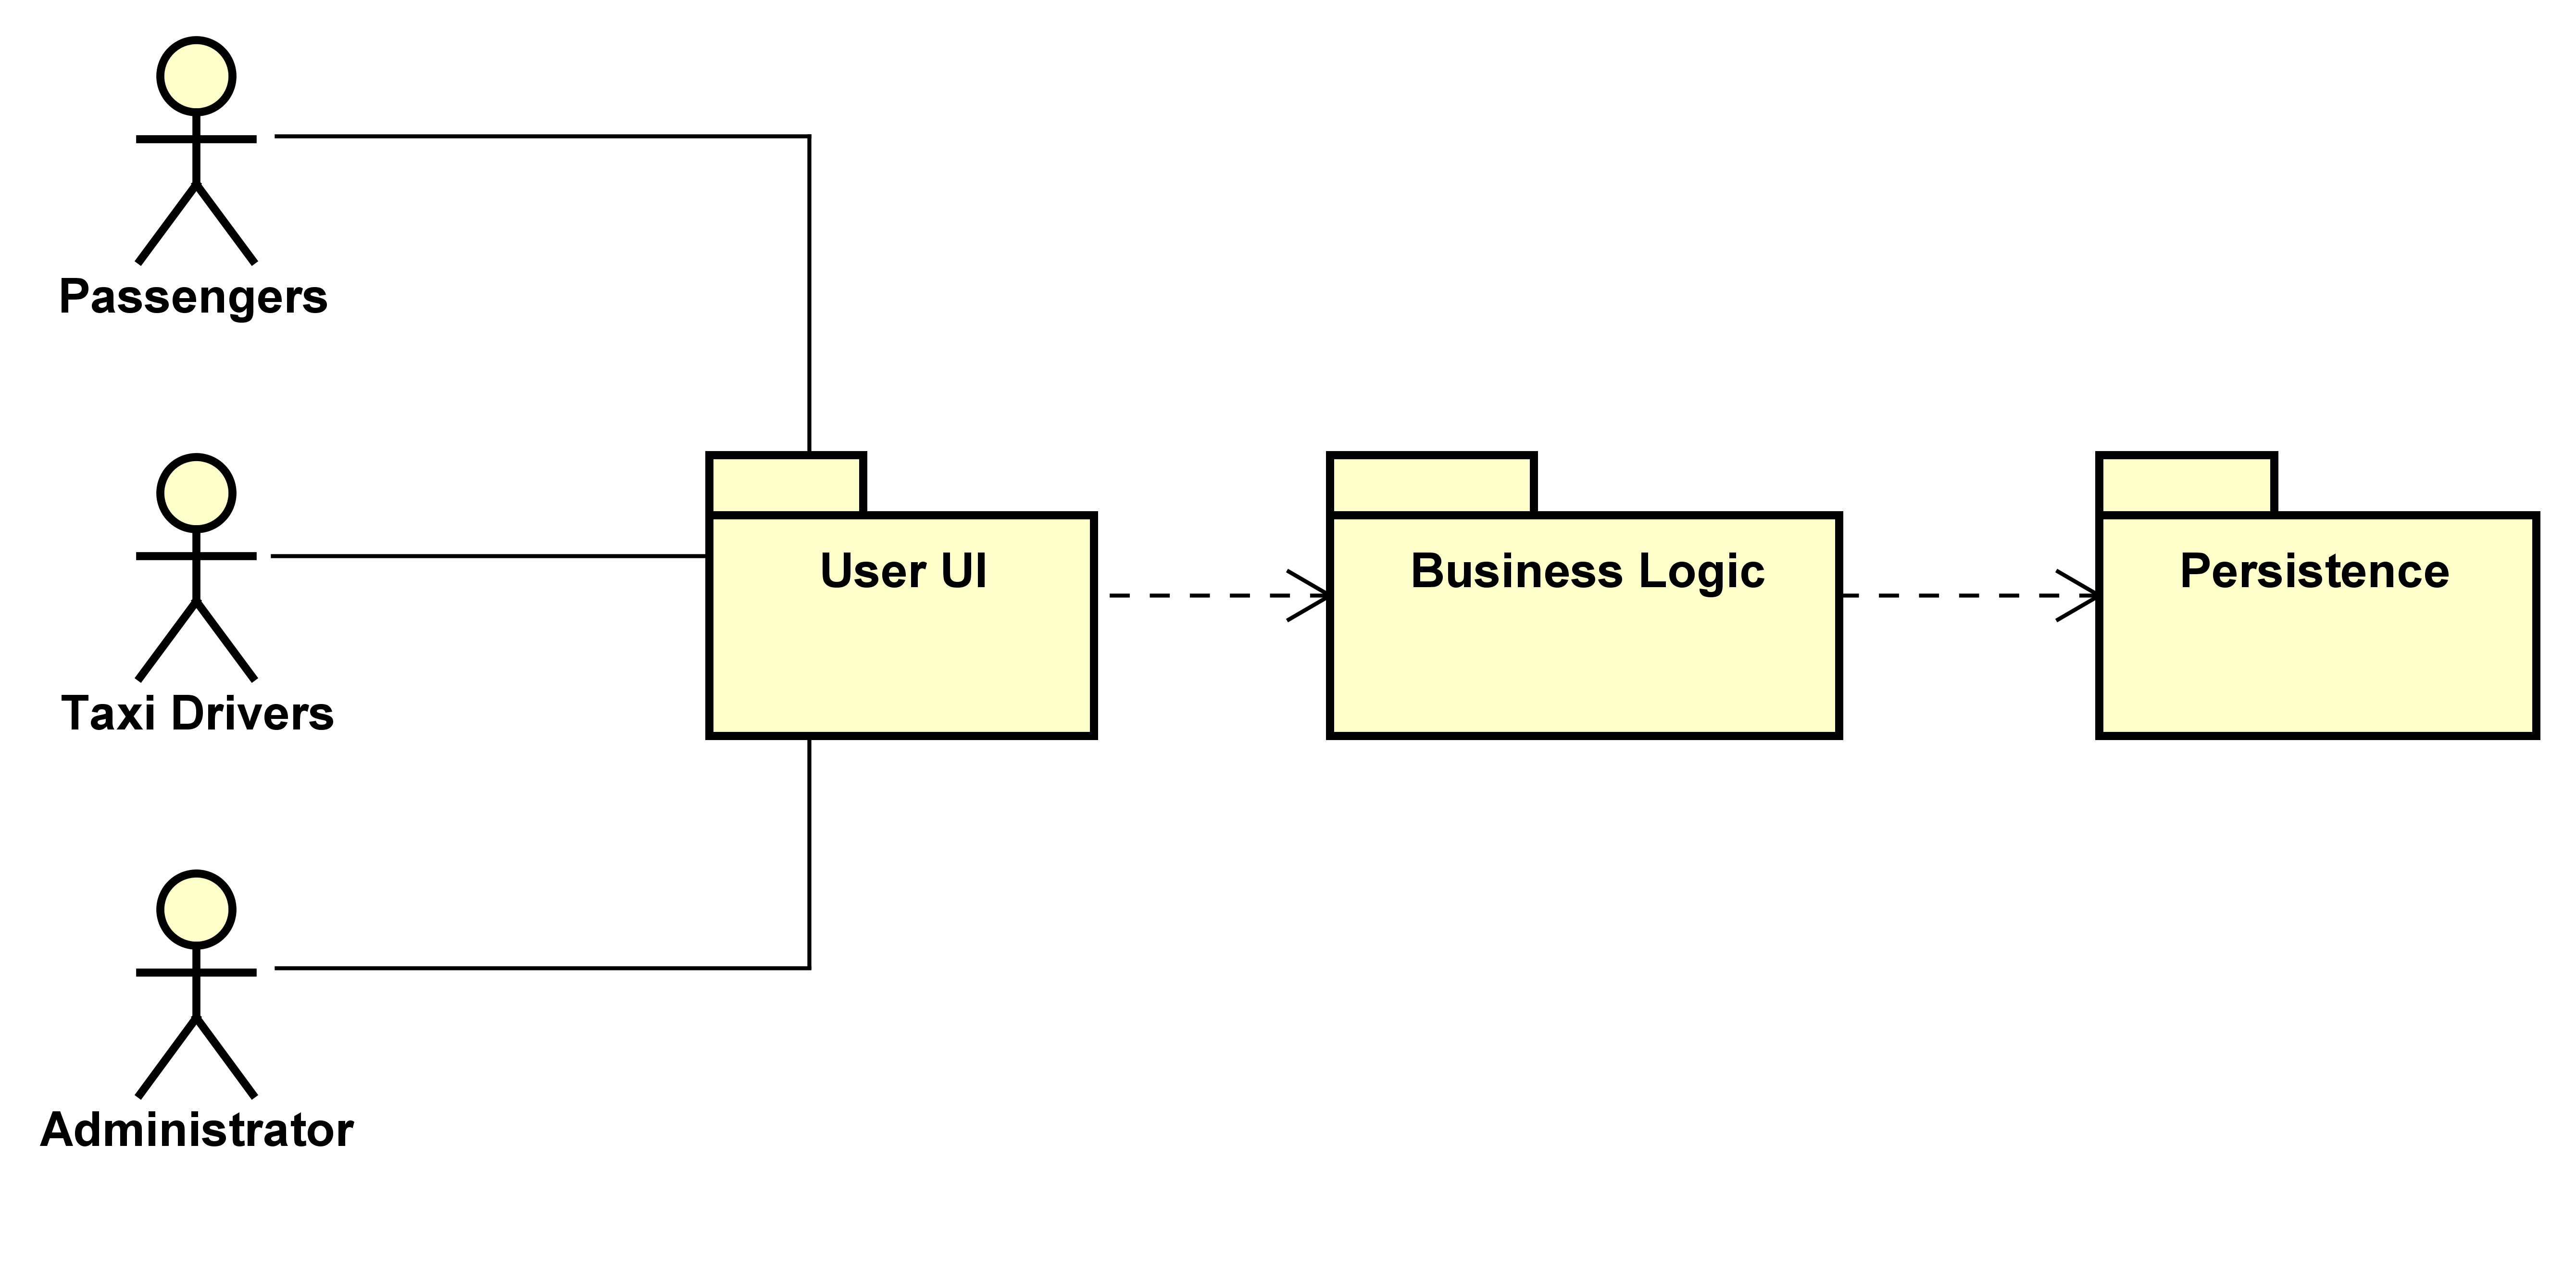
\includegraphics[keepaspectratio=true,scale=0.6]{Pictures/Packages}}
%	\end{minipage}	
	
	
	\subsection{Component view}
%	The inner packages are described as follows:\\
%	\begin{itemize}
%		\item User UI:	this set of sub-packages is responsible for encapsulating the user's actions and forwarding information requests to the Business Logic sub-packages.
%		\item Business logic: this set of sub-packages is responsible for handling requests from the User UI package, processing them and sending back a response. These packages may access the Persistence package.
%		\item Persistence: this set of sub-packages contains the data model for the system. It accepts requests from the Business Logic package.
%	\end{itemize}
%	A more detailed view of the system:\\
%	\begin{minipage}{\linewidth}
%%		\vspace*{-0.35cm}
%		\makebox[\linewidth]{
%		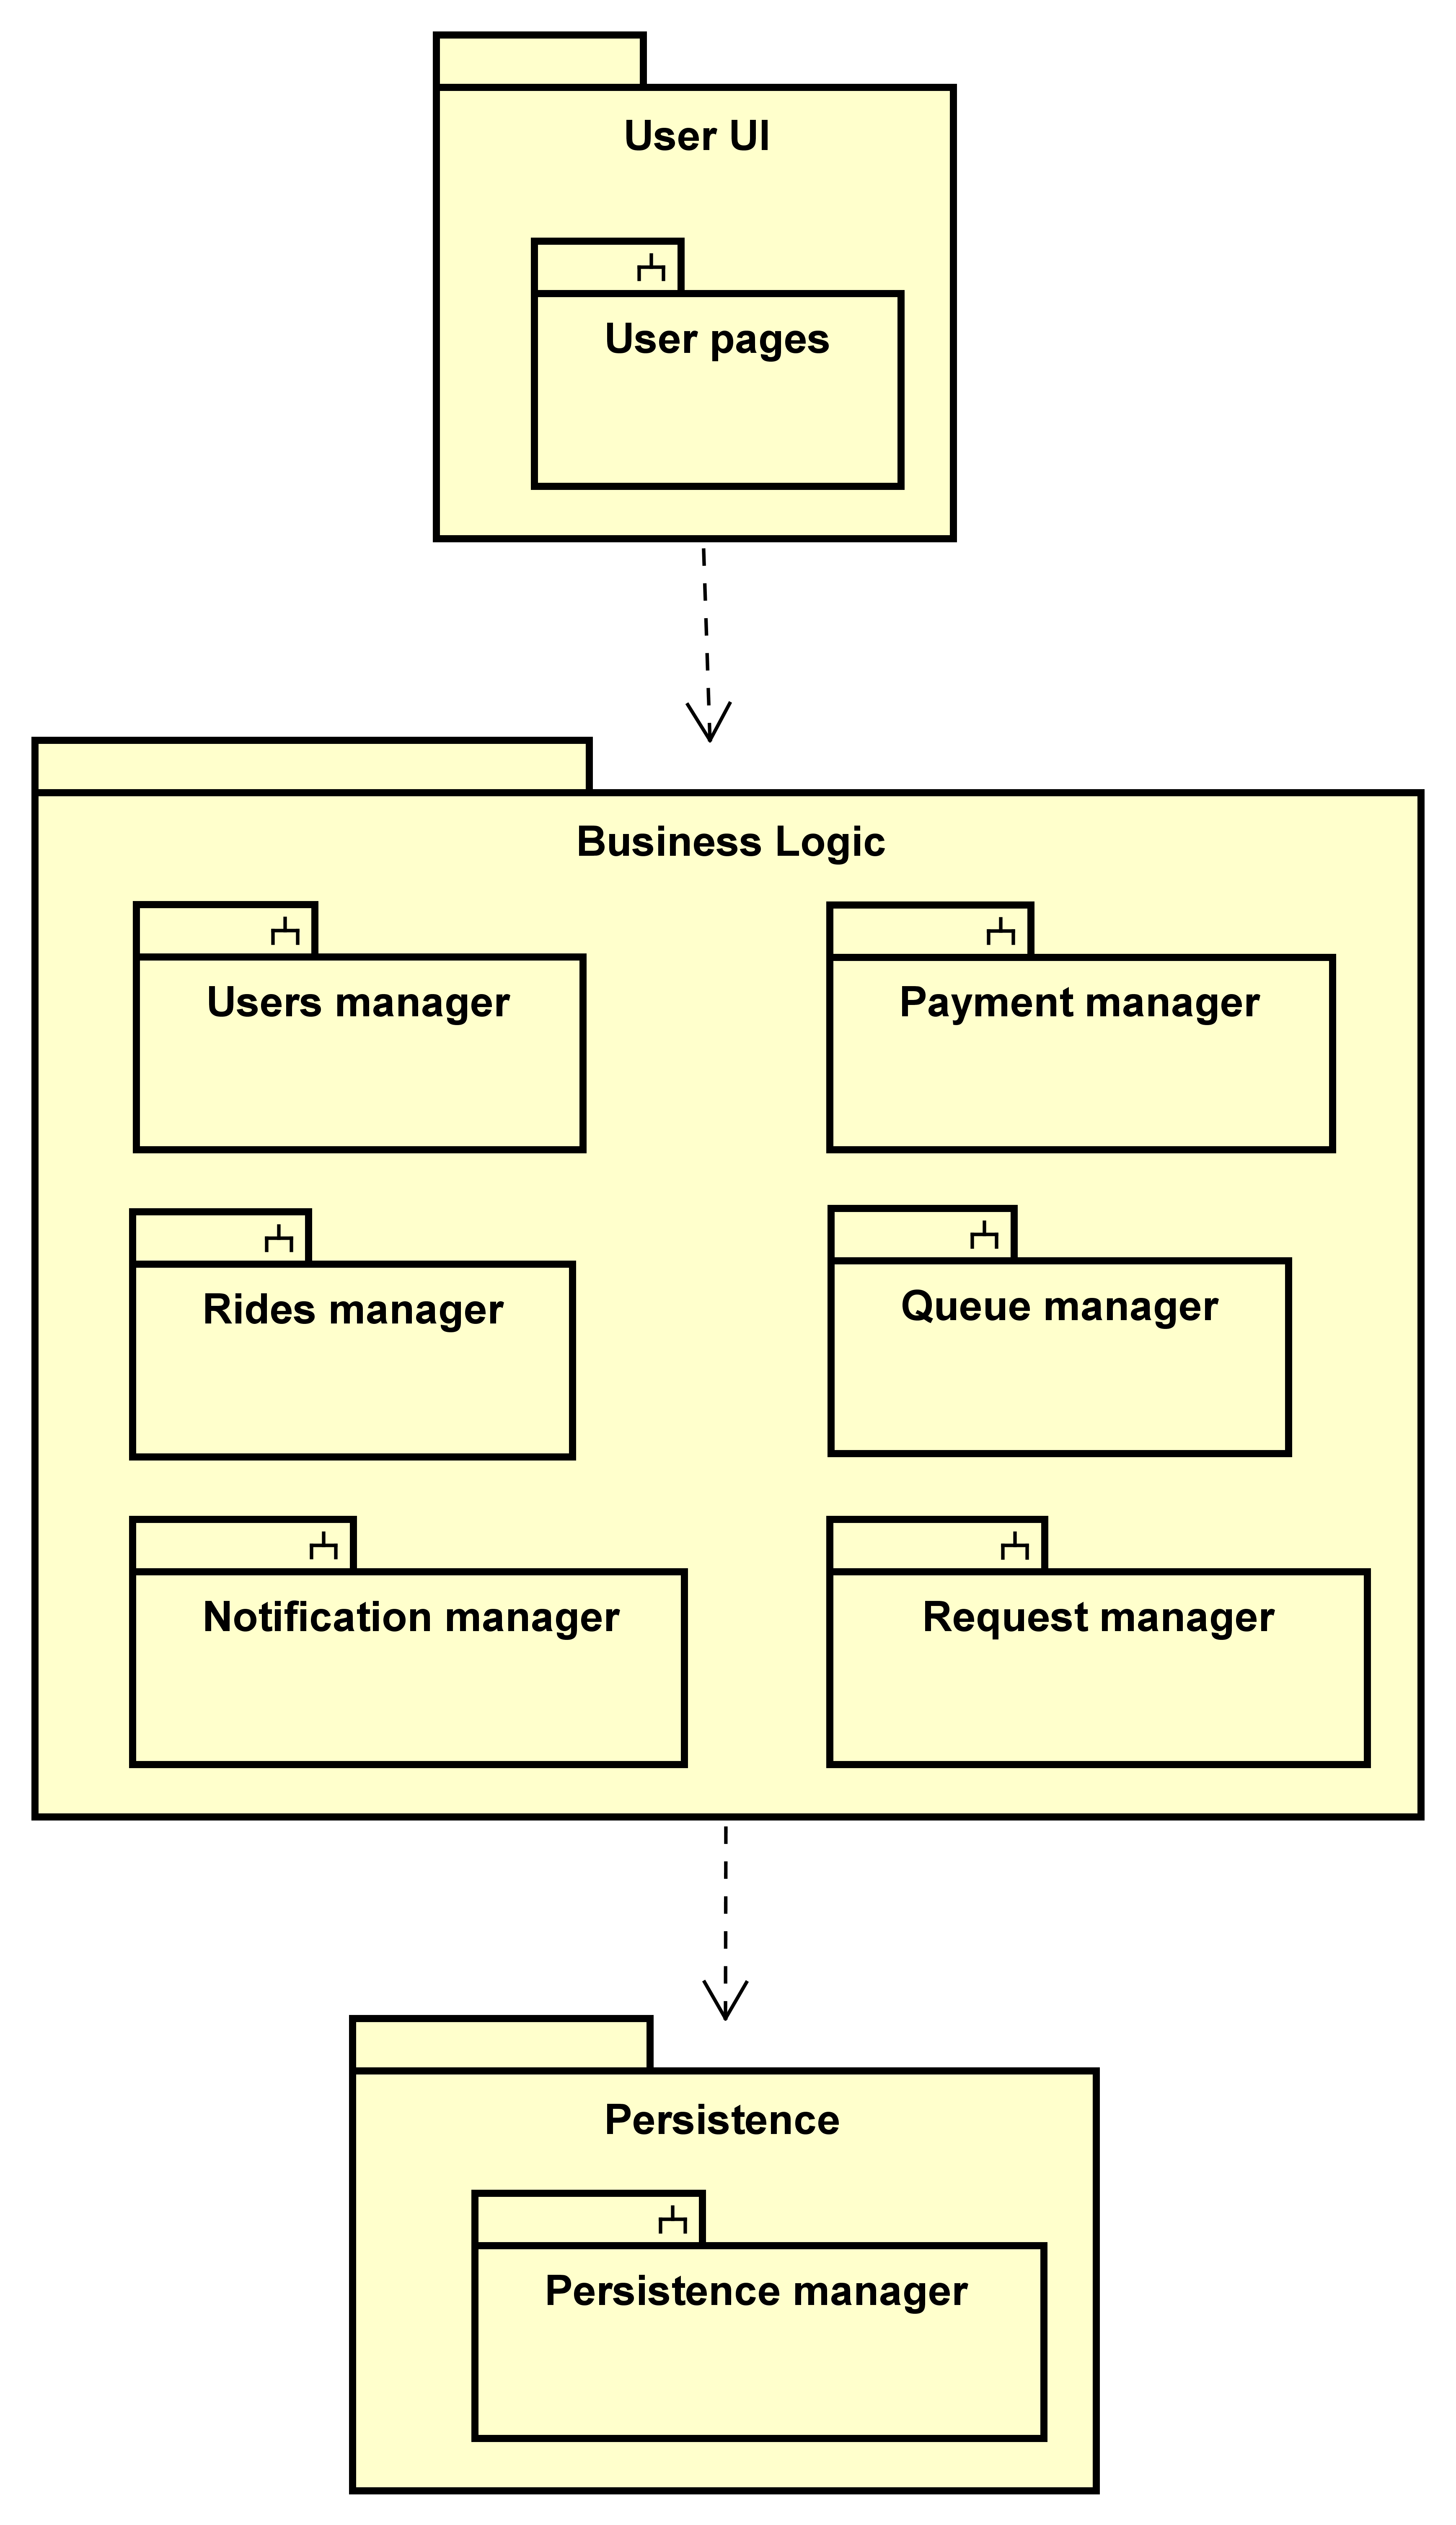
\includegraphics[keepaspectratio=true,scale=0.8]{Pictures/PackagesDetails}}
%	\end{minipage}

	\begin{minipage}{\linewidth}
%		\vspace*{-0.35cm}
		\makebox[\linewidth]{
		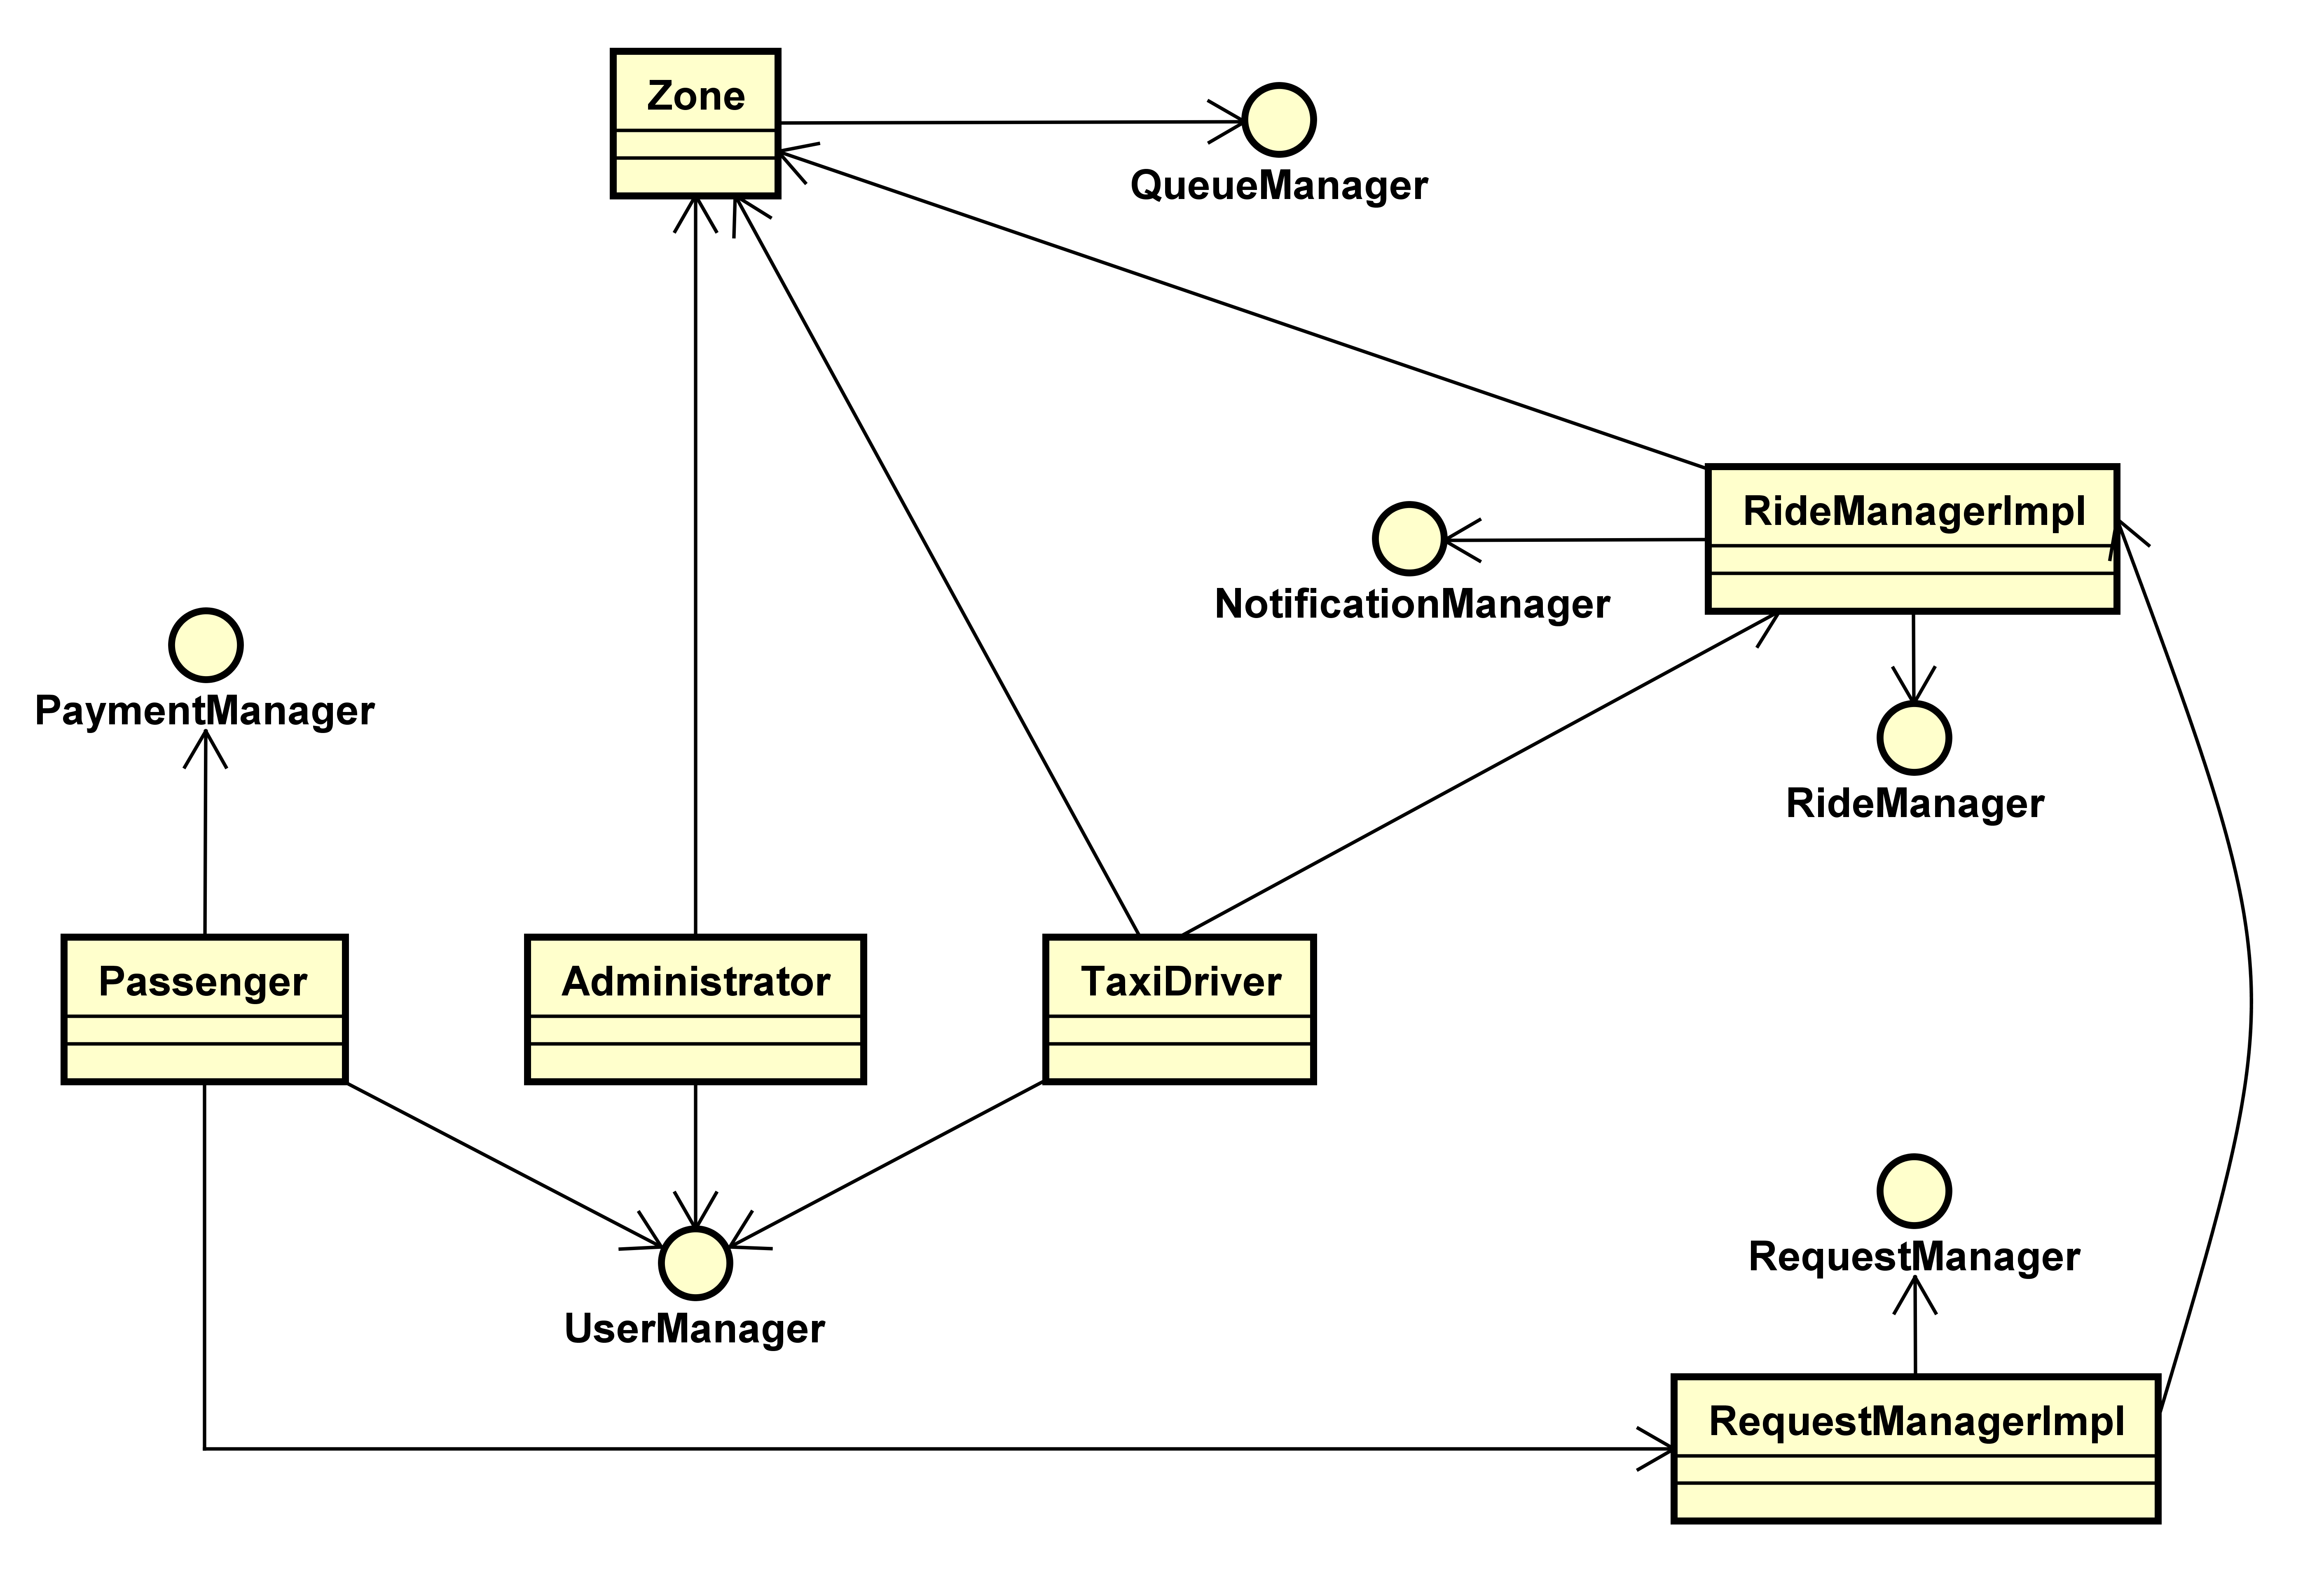
\includegraphics[keepaspectratio=true,scale=0.7]{Pictures/ComponentView}}
	\end{minipage}	

	
	
	\subsection{Deployment view}
	
	\subsection{Runtime view}
	
	\subsection{Component interfaces}
	
	\subsection{Selected architectural styles and patterns}
	
	\subsection{Other design decisions}

	\section{Algorithm design}
	
	\section{User Interface Design}
	
	\section{Requirements Traceability}
	
	\section{References}
	
	\section{Appendix}
	
	\subsection{Software and tools used}
	\begin{itemize}
		\item TeXstudio 2.10.4 (http://www.texstudio.org/) to redact and format this document.
		\item Astah Professional 7.0 (http://astah.net/editions/professional): to create Use
		Cases Diagrams, Sequence Diagrams, Class Diagrams and State Machine	Diagrams.
		\item Microsoft Office Visio Professional 2016
%		\item Balsamiq Mockups 3.2.4 (http://balsamiq.com/products/mockups/) to create the mockups.
	\end{itemize}
	
	\subsection{Hours of work} The time spent to redact this document:
	\begin{itemize}
		\item Baldassari Alessandro: 35 hours.
		\item Bendin Alberto: 35 hours.
		\item Giarola Francesco: 35 hours.
	\end{itemize}
\end{document}